\subsection{Generación de trayectorias}
La semana 8 construye trayectorias articulares a partir de condiciones en los extremos \parencite{course8}. Para $u=t/T$, $\Delta q=q_f-q_i$ y $0\leq t\leq T$:
\begin{align}
q_3(t)&=q_i+\Delta q(3u^2-2u^3),\\
q_5(t)&=q_i+\Delta q(10u^3-15u^4+6u^5).
\end{align}
Los subíndices 3 y 5 indican el orden del polinomio, no una articulación. Ambos imponen velocidad nula al inicio y al final; el quíntico impone además aceleración nula. Se obtienen $\dot q$ y $\ddot q$ por derivación analítica.

El ejemplo emplea $q_i=(30,40,-50)^\circ$, $q_f=(-20,20,-70)^\circ$ y $T=3$ s, convertidos a radianes para calcular. No se mezclan funciones trigonométricas en grados con derivadas expresadas en radianes. La trayectoria cartesiana se obtiene por directa y no tiene por qué ser una recta.
\begin{figure}[htbp]\centering
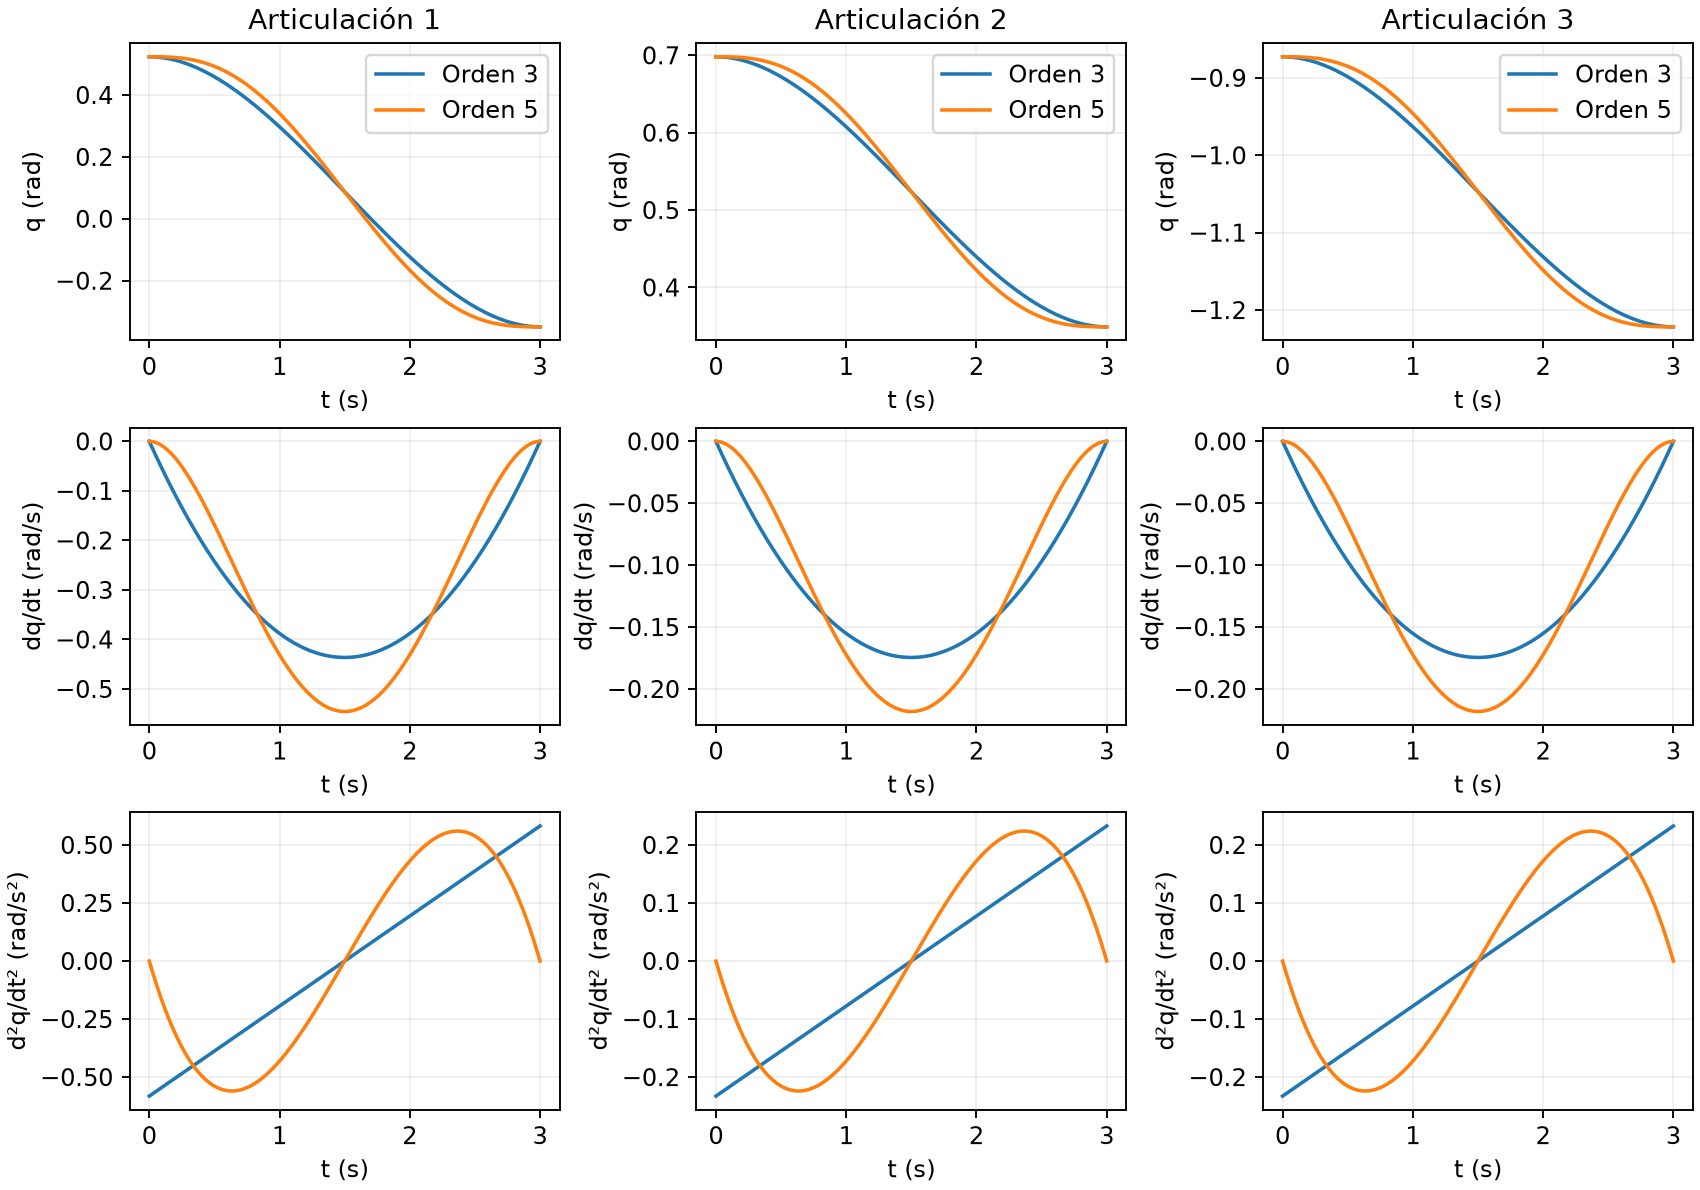
\includegraphics[width=\linewidth]{../simulations/course/results/run-001/interpolation.png}
\caption{Posición, velocidad y aceleración por articulación para interpoladores cúbico y quíntico.}
\end{figure}
